%% -*- mode: latex; mode: flyspell -*-
\documentclass[12pt, letter]{article}

%% Class name and Assignment number
%%
\newcommand{\courseName}{CSC421: Artificial Intelligence}
\newcommand{\assignName}{Assignment~3}

%% Packages
\usepackage{amsmath,amsfonts,amssymb,amsthm,dsfont}
\usepackage{physics}
\usepackage{graphicx}
\usepackage[bookmarks=false]{hyperref}
\usepackage{color}
\usepackage{lipsum}
\usepackage{placeins}
\usepackage{float}
\restylefloat{table}

%% Paper format
\usepackage{geometry}
\geometry{
    letterpaper,
    %% total={216mm,279mm}, %< NSERC size
    margin=2.00cm,     %< default
    %% margin=1.87cm,       %< NSERC tightest
}

%% Headers and footers
\usepackage[explicit]{titlesec}
\newpagestyle{titlesec_assignment}{
  \sethead{\courseName}{}{\assignName}\setfoot{}{\thepage}{}
  \headrule
  %% \footrule
}

\begin{document}

%% Set header and footer
\pagestyle{titlesec_assignment}

%% Title
\title{\courseName\\\assignName}
\author{Rafael Solorzano}
\maketitle

\section{Introduction}

In this assignment CSP problems solving using python-csp is explored. Two different problems are solved, the first being a Crypto-arithmetic puzzle and the second being the Waltz Filtering problem. Further, a Naive Bayes Text Classification is computer similar to the movie classification done in Assignment 2, but this time the entire computation is done using scikit-learn. Finally, usage of pgmpy to create Bayesian Networks and get results is done.  

\section{CSP}

\subsection{Crypto-arithmetic Puzzle}

The crypto-arithmetic puzzle solved in this problem consists of finding a consistent assignment for the sum of TWO + TWO = FOUR in which each letter is assigned a number and the result of each letter produces FOUR. The problem is solved using python-csp and yields several results which are shown in Figure 1. Further the code is shown in Figure 2. The python-csp is used by first creating a problem object and further assigning variables and its corresponding domain.Second, the constraints of the problem are specified; for this specific problem all the main variables must be non-equal therefore they are assigned as so, further the other constraint that is added is the summation result of each variable, according to the problem definition. Finally, the solutions of the problem are printed. 

 \begin{figure}[htb]
  \centering
  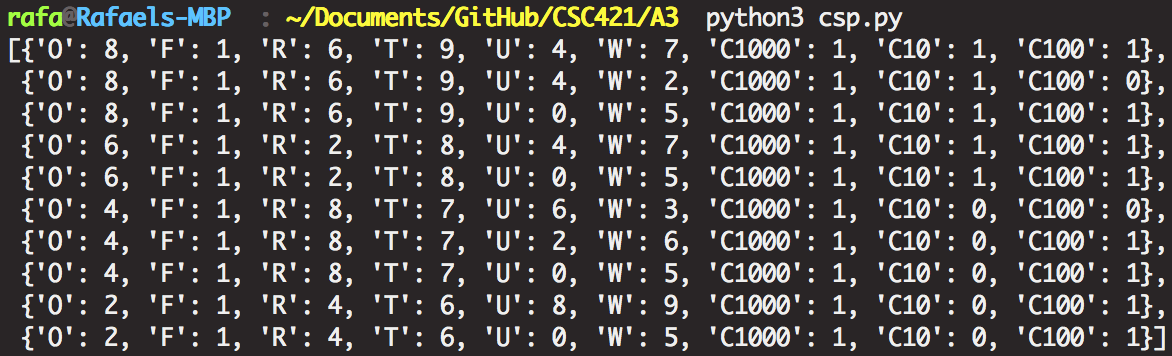
\includegraphics[width=0.75 \textwidth]{./figures/csp_results.png}
  \caption{The solutions for the crypto puzzle.}
\end{figure}

 \begin{figure}[htb]
  \centering
  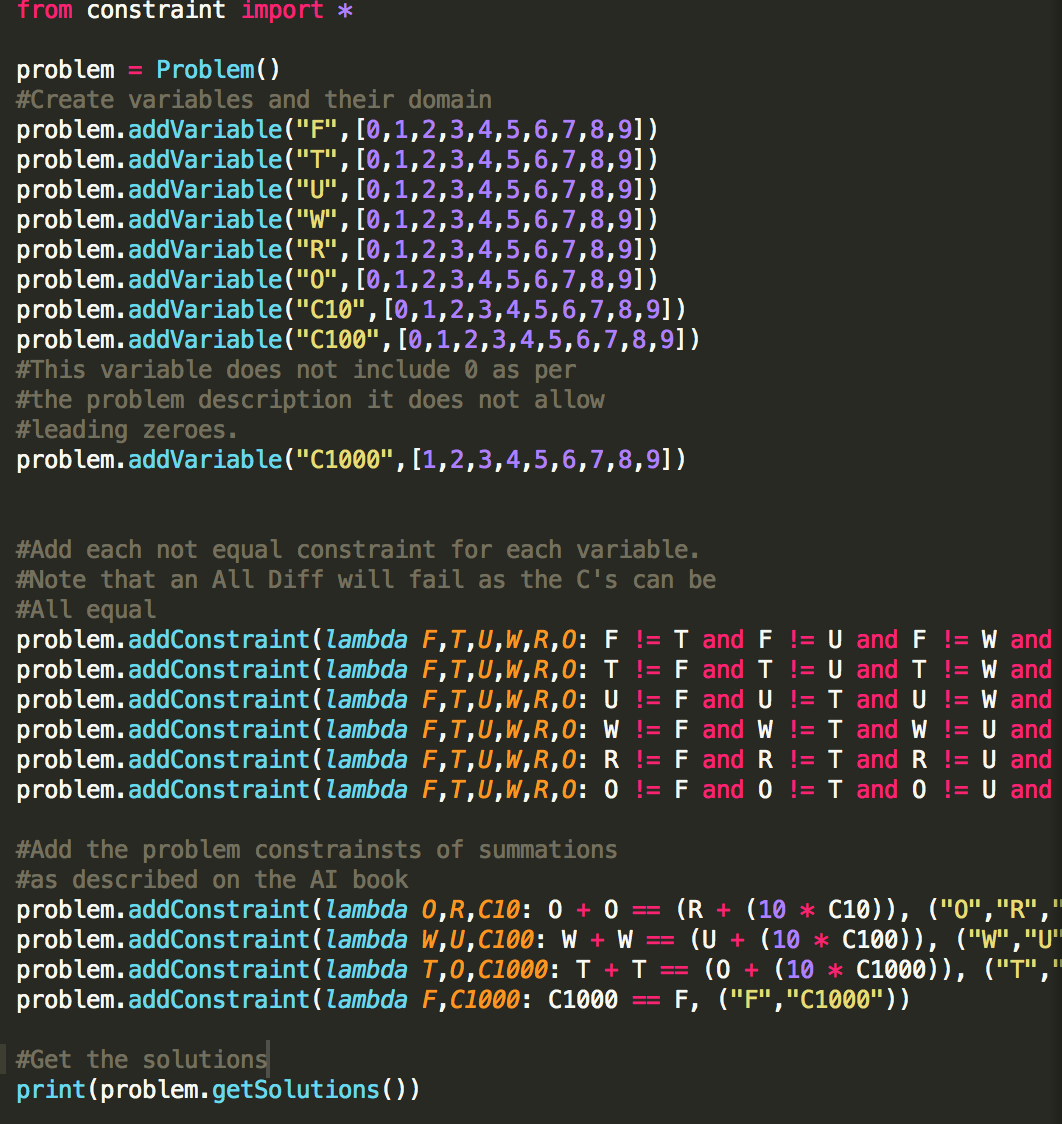
\includegraphics[width=0.80 \textwidth]{./figures/csp_code.png}
  \caption{The code that solves the crypto puzzle.}
\end{figure}

\FloatBarrier

\subsection{Waltz Filtering}

\section{Naive Bayes Text Classification}

Note that in this problem additionally to the  the 10-fold cross validation i compared this against a train test split of 25\% saved for testing. The results of both are presented in this section. 

In this problem text classification of movies reviews that are classified in negative and positive is done using scikit-learn. First, the reviews text files are loaded directly using scikit feature extraction text functions, further the categories detected by scikit, which are based on folder names are printed, this is done for the sole purpose of checking if the correct folders were interpreted. This code is shown in Figure 3.

Once, the text is processed Pipelines for their classification using Multinomial and Bernoulli Naive Bayes are created. This pipelines are shown in Figure 4. Further, the test and train split is created, and accuracy is calculated using this method for both Bayes classifiers. Finally, the 10-fold cross-validation is performed using both classifiers. The code for both this methods is shown in Figure 5, whereas their results are shown in Figure 6, note that the best accuracy was achieved using the 10-fold cross validation with Multinomial NB. 

 \begin{figure}[htb]
  \centering
  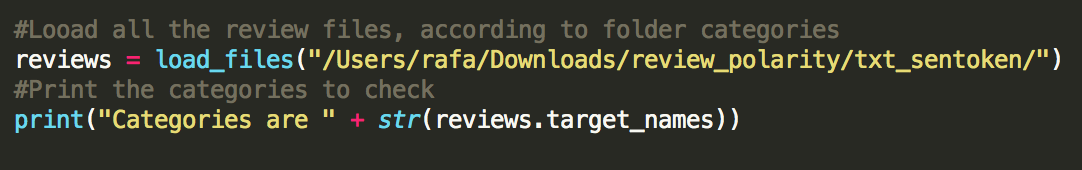
\includegraphics[width=0.75 \textwidth]{./figures/file_load.png}
  \caption{Loading the movie reviews txt files.}
\end{figure}

 \begin{figure}[htb]
  \centering
  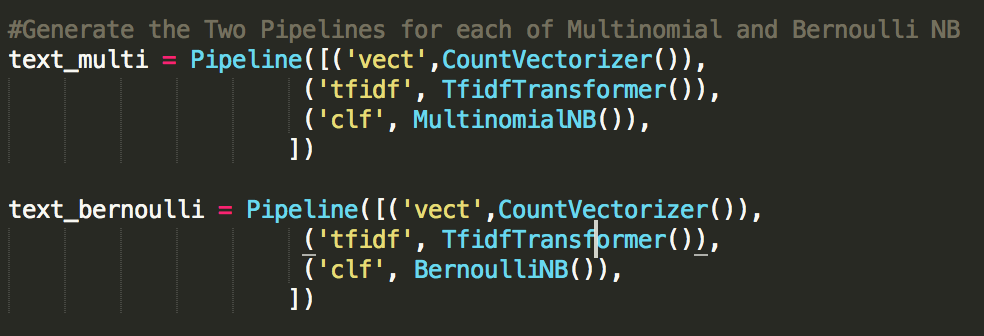
\includegraphics[width=0.75 \textwidth]{./figures/pipeline.png}
  \caption{Pipelines for Multinomial and Bernoulli NB.}
\end{figure}

 \begin{figure}[htb]
  \centering
  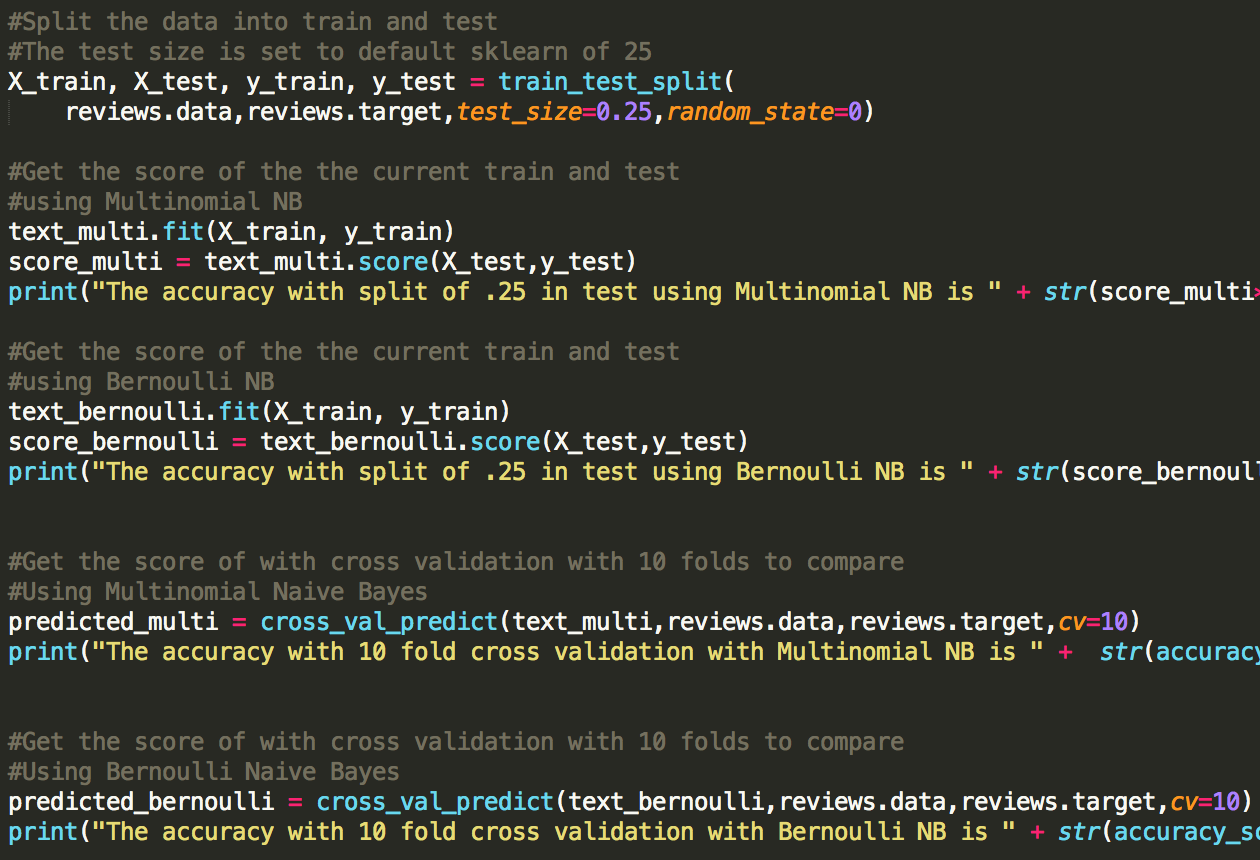
\includegraphics[width=0.85 \textwidth]{./figures/text_tests.png}
  \caption{Performing the classification, with test-train split and cross-validation.}
\end{figure}

 \begin{figure}[htb]
  \centering
  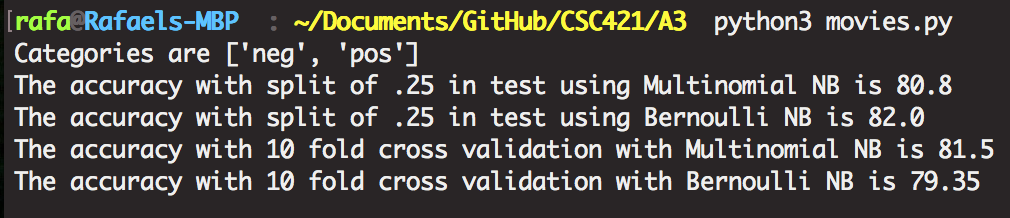
\includegraphics[width=0.75 \textwidth]{./figures/text_result.png}
  \caption{All the results of test-train and cross-validation using both Multinomial and Bernoulli NB.}
\end{figure}

\FloatBarrier


\section{Discrete Bayesian Networks}

In this section pgmpy is used to create a Bayesian Network. First, the Bayesian model is created, that indicated the connections between nodes. Further, the probabilities distribution of each node is specified using TabularCPD in which the variable name being specified, the number of variable cards it's values, it's evidence, and the evidence\_card is specified. The code that creates this tables is shown in Figure 7. Further an example printout of a table is shown in Figure 8. Once the CPDs have been created they are added to the model, once this is done an inference object can be created to perform inference

The query provided as example in the assignment can be computed by using inference step by step. The code that achieves this is shown in Figure 9, whereas the result is shown in Figure 10. Note that pgmpy returns a Discrete Factor object that prints to a table containing all probabilities related to the query, it is easy to find the required values in each table. 

Finally, when we want to know how likely George is to get a strong recommendation letter we do it with inference as well. This yields a result of 56.8\%. Further if we want to know the same probabilities but know we know that George is not a strong musician this is also is done by inference, and yields a results of 65.1\%. The code that infers the data is shown in Figure 11, whereas its results are shown in Figure 12, in order. 

Note that this may seem non-sensical but as it has been mentioned in lecture and announcements the data is non-sensical and is only for demonstration of usage of the pgmpy library further, the results do not match assignment 3 results in the description as it was also mentioned that the results provided in the assignment are wrong and there was no easy way to fix them to provide correct results for comparison.

 \begin{figure}[htb]
  \centering
  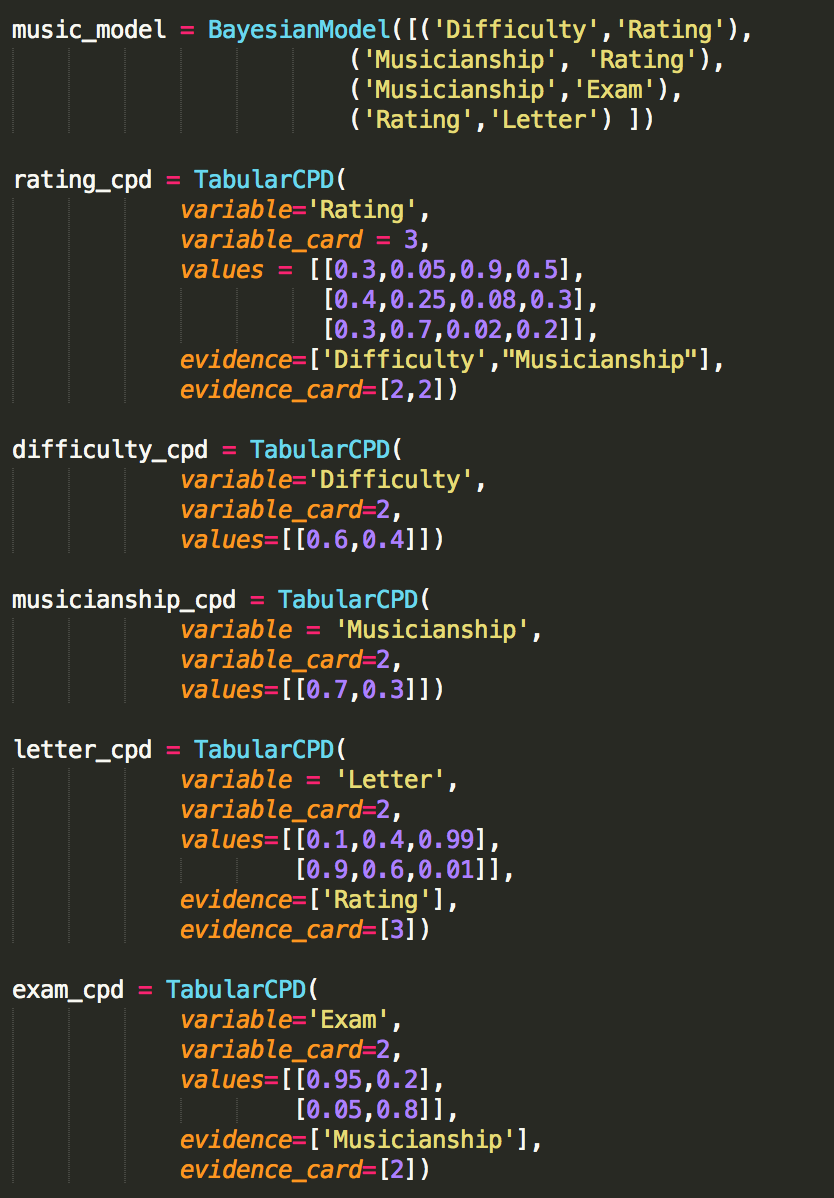
\includegraphics[width=0.75 \textwidth]{./figures/bayesian_create.png}
  \caption{Creating the Bayesian Network structure.}
\end{figure}

 \begin{figure}[htb]
  \centering
  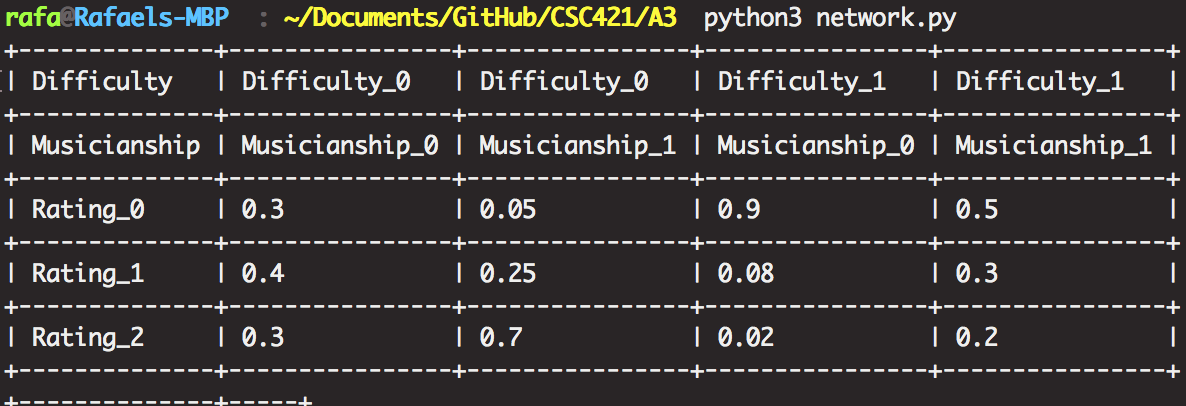
\includegraphics[width=0.75 \textwidth]{./figures/table_example.png}
  \caption{An example table created with TabularCPD.}
\end{figure}

 \begin{figure}[htb]
  \centering
  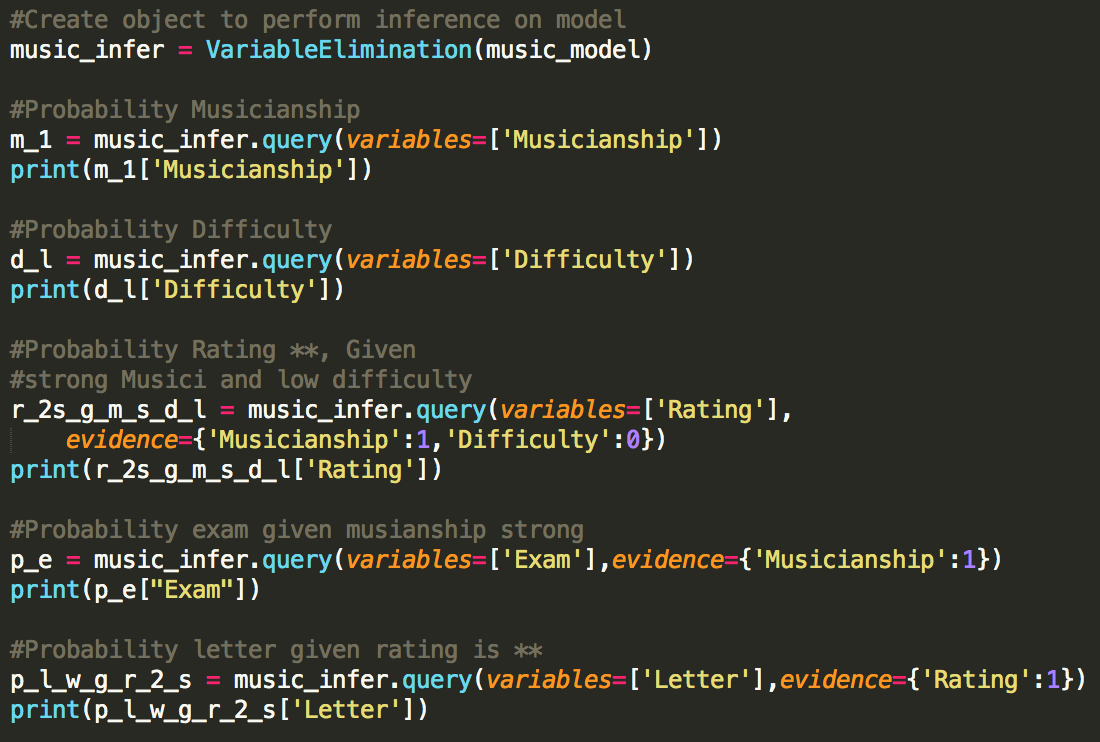
\includegraphics[width=0.80 \textwidth]{./figures/inference_problem.png}
  \caption{Performing inference, according to assignment problem.}
\end{figure}

 \begin{figure}[htb]
  \centering
  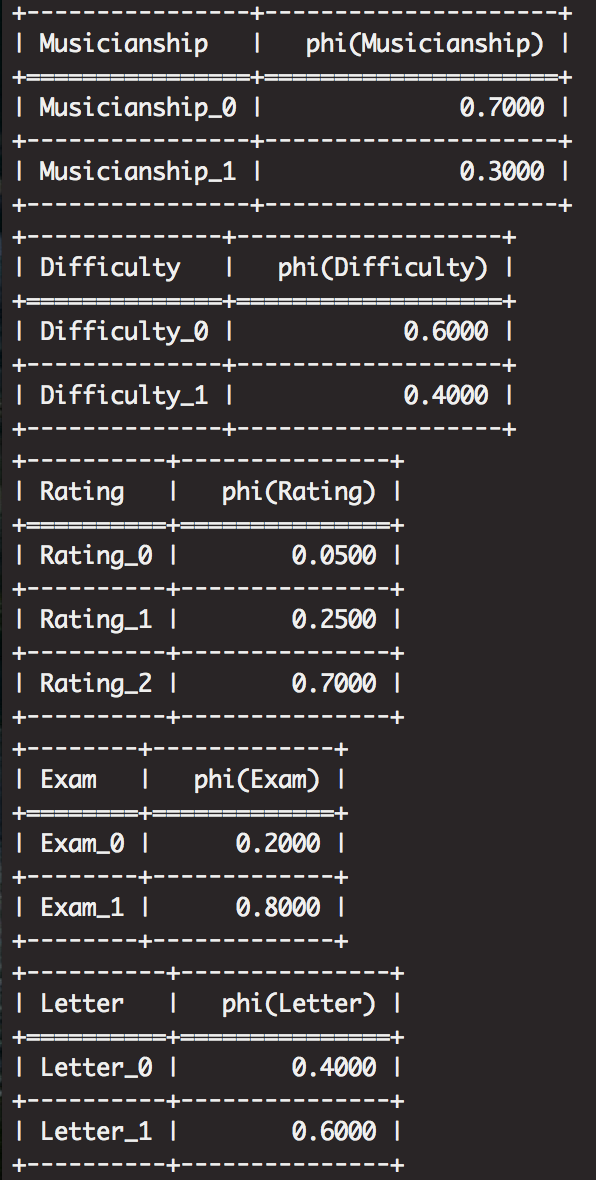
\includegraphics[width=0.50 \textwidth]{./figures/inference_result.png}
  \caption{All the results of performing inference.}
\end{figure}

 \begin{figure}[htb]
  \centering
  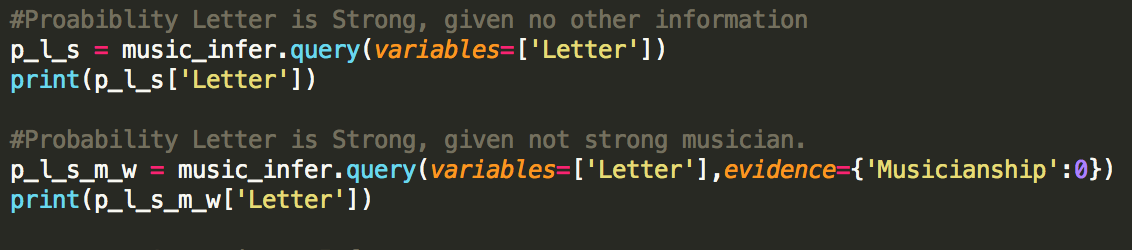
\includegraphics[width=0.80 \textwidth]{./figures/george.png}
  \caption{Performing inference to test strong letter of recommendation.}
\end{figure}

 \begin{figure}[htb]
  \centering
  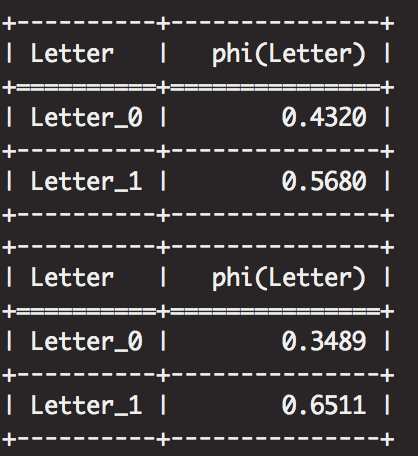
\includegraphics[width=0.50 \textwidth]{./figures/george_result.png}
  \caption{The result of the strong letter of recommendation.}
\end{figure}

\FloatBarrier

\subsection{Approximation Inference}

Approximate Inference was attempted with pgmpy by using MPLP. Max-Product Linear Programming uses a Markov Model for inference so the Bayesian Network is first transformed into a Markov Model using the built in pgmpy function. Sadly, this produced an error, that is caused by either the implementation of MPLP or the transferring of my Bayesian Network into Markov Model. Nevertheless, the code is shown in Figure 13, with the resultant error in Figure 14. The expected result of the last map\_query function would be a dictionary of the best assignment of the nodes in a form of a dictionary. 

 \begin{figure}[htb]
  \centering
  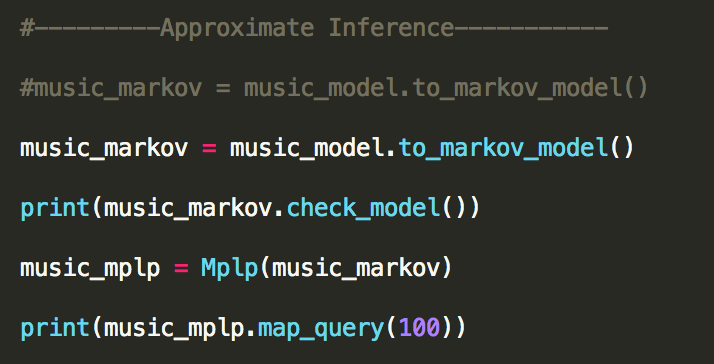
\includegraphics[width=0.6 \textwidth]{./figures/approximate_inference.png}
  \caption{Attempt at approximate inference.}
\end{figure}

 \begin{figure}[htb]
  \centering
  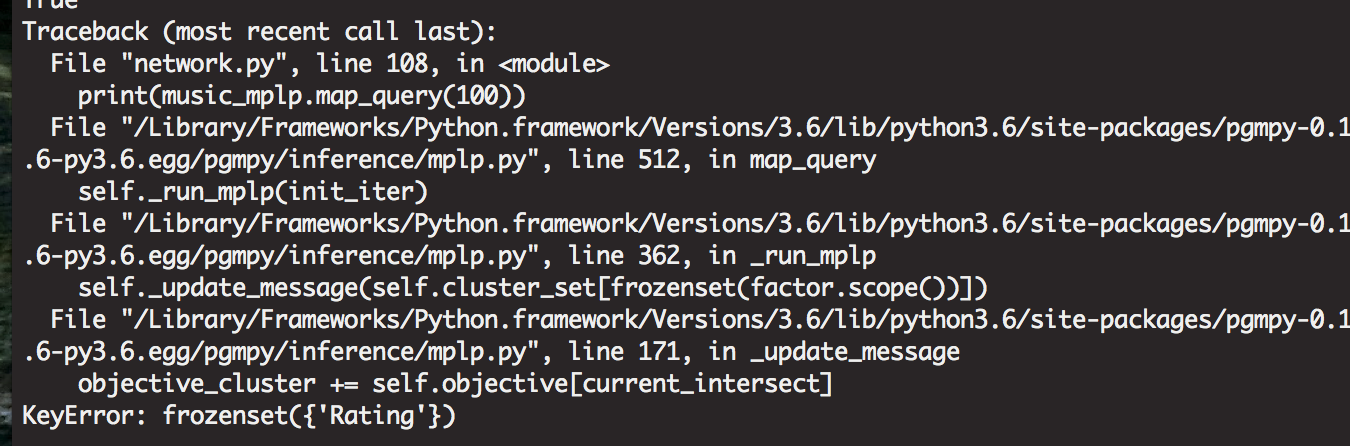
\includegraphics[width=0.75 \textwidth]{./figures/error_approx.png}
  \caption{Resulting error from approximate inference code.}
\end{figure}

\FloatBarrier

\end{document}



%%% Local Variables:
%%% mode: latex
%%% TeX-master: t
%%% End:
